\section{Data Release Production}
\label{sec:drp}

\begin{figure}
\centering
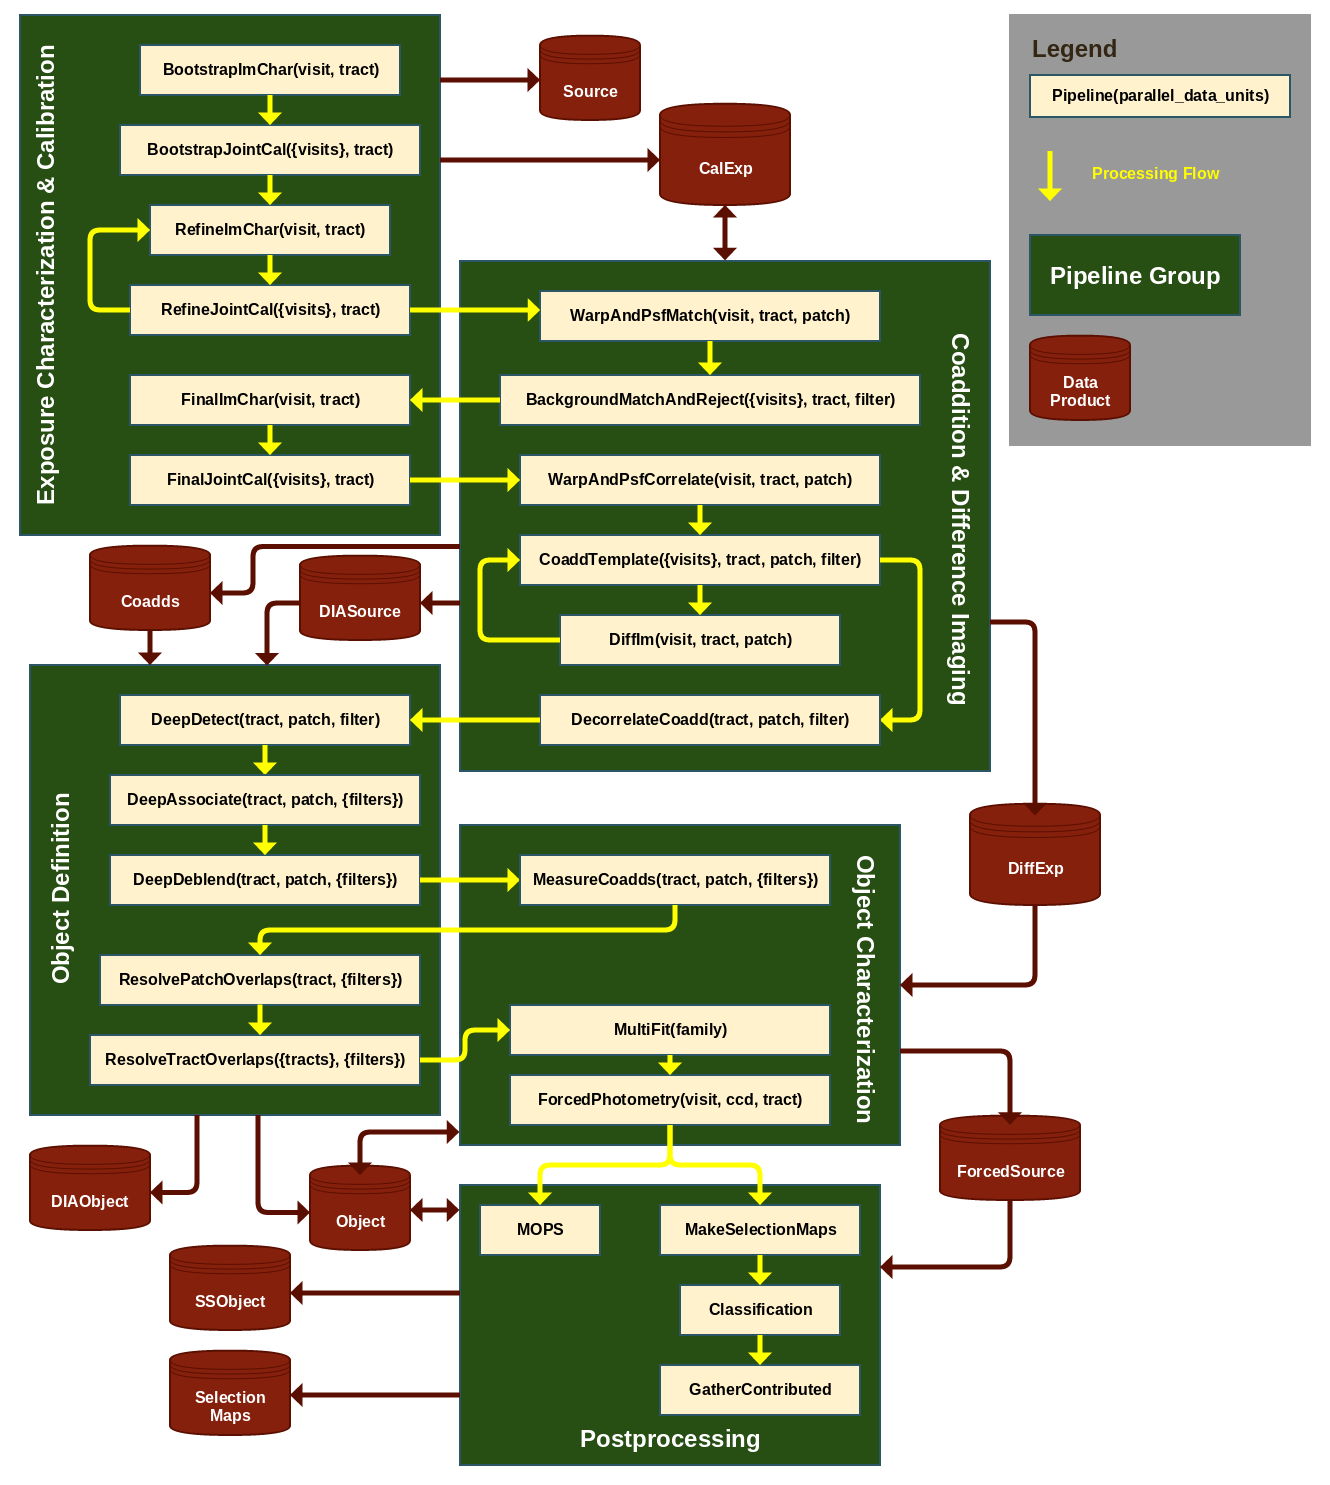
\includegraphics[width=\textwidth]{figures/drp_summary.png}
\caption{Summary of the Data Release Production processing flow.  Processing is split into multiple pipelines, which are conceptually organized into the groups discussed in sections~\ref{sec:drp_imchar_and_jointcal}-\ref{sec:drp_postprocessing}.
\label{fig:drp_summary}}
\end{figure}

A Data Release Production is run every year (twice in the first year of operations) to produce a set of catalog and image data products derived from all observations from the beginning of the survey to the point the production began.  This includes running a variant of the difference image analysis run in Alert Production, in addition to direct analysis of individual exposures and coadded images.  The data products produced by a Data Release Production are summarized in table~\ref{table:drp_data_products}.


\begin{table}
\small
\begin{tabularx}{\textwidth}{ | l | l | X | }
  \hline
  {\bf Name} & {\bf Availability} & {\bf Description} \\
  \hline
  Source & Stored &
  Measurements from direct analysis of individual exposures. \\
  \hline
  DIASource & Stored &
  Measurements from difference imagine analysis of individual exposures. \\
  \hline
  Object & Stored &
  Measurements for a single astrophysical object, derived from all available information, including coadd measurements, simultaneous multi-epoch fitting, and forced photometry.  Does not include solar system objects. \\
  \hline
  DIAObject& Stored &
  Aggregate quantities computing by associating spatially colocated DIASources. \\
  \hline
  ForcedSource & Stored &
  Flux measurements on each direct and difference image at the position of every Object. \\
  \hline
  SSObject & Stored &
  Solar system objects derived by associating DIASources and inferring their orbits. \\
  \hline
  CalExp & Regenerated &
  Calibrated exposure images for each CCD/visit (sum of two snaps). \\
  \hline
  DiffExp & Regenerated &
  Difference between CalExp and PSF-matched template coadd. \\
  \hline
  DeepCoadd & Stored &
  Coadd image with a reasonable combination of depth and resolution. \\
  \hline
  EpochRangeCoadd & Renegerated &
  Coadd image that cover only a limited range of epochs. \\
  \hline
  BestSeeingCoadd & Regenerated &
  Coadd image built from only the best-seeing images. \\
  \hline
  PSFMatchedCoadd & Regenerated &
  Coadd image with a constant, predetermined PSF. \\
  \hline
\end{tabularx}
\caption{Table of public data products produced during a Data Release Production.  A full description of these data products can be found in the Data Products Definition Document (LSE-163).
\label{table:drp_data_products}}
\end{table}

From a conceptual standpoint, data release production can be split into five groups of pipelines, executed in approximately the following order:
\begin{enumerate}
\item We characterize and calibrate each exposure, estimating point-spread functions, background models, and astrometric and photometric calibration solutions.  This iterates between processing individual exposures independently and jointly fitting catalogs derived from multiple overlapping exposures.  These steps are described more fully in section~\ref{sec:drp_imchar_and_jointcal}.
\item We alternately combine images and subtract them, using differences to find artifacts and time-variable sources while building coadds that produce a deeper view of the static sky.  Coaddition and difference imaging is described in section~\ref{sec:drp_coaddition_and_diffim}.
\item We detect and deblend on coadds, while associating these detection with detections from difference imaging to define objects.  We then merge catalogs in the overlap regions between patches and tracts to produce a single contiguous catalog over the full sky.  This is described in section~\ref{sec:drp_object_definition}.
\item We measure objects on coadds and visit-level direct and difference images in object characterization, as described section~\ref{sec:drp_object_characterization}.
\item After all image processing is complete, we run additional catalog-only pipelines to fill in additional object properties.  Unlike previous stages, this postprocessing is not localized on the sky, as it may use statistics computed from the full data release to improve our characterization of individual objects.  Postprocessing pipelines are described in section~\ref{sec:drp_postprocessing}.
\end{enumerate}
This conceptual ordering is an oversimplification of the actual processing flow, however; as shown in Figure~\ref{fig:drp_summary}, pipeline groups are actually interleaved.

Each pipeline in this the diagram represents a particular piece of code excuted in parallel on a specific unit of data, but pipelines may contain additional (and more complex) parallelization to further subdivide that data unit.  The processing flow also includes the possibility of iteration between pipelines, indicated by cycles in the diagram.  The number of iterations in each cycle will be determined (via tests on smaller productions) before the start of the production, allowing us to remove these cycles simply by duplicating some pipelines a fixed number of times.  The final data release production processing can thus be described as a directed acyclic graph (DAG) to be executed by the orchestration middleware, with pipelines as edges and (intermediate) data products as vertices.  Most of the graph will be generated by applications code before the production begins, using a format and/or API defined by the orchestration middleware.  Howver, some parts of the graph must be generated on-the-fly; this will be discussed further in section~\ref{sec:drpMultiFit}.


\subsection{Exposure Characterization and Calibration}
\label{sec:drp_imchar_and_jointcal}

\begin{note}[ImChar/JointCal Diagram]
Extract ImChar/JointCal pipelines from ``DRP Top-Level Overview'' on confluence and expand detail to show data flow and ordering of ``Task/Process'' boxes.
\end{note}

\subsubsection{BootstrapImChar}
\label{sec:drpBootstrapImChar}
\subsubsection{BootstrapJointCal}
\label{sec:drpBootstrapJointCal}
\subsubsection{RefineImChar}
\label{sec:drpRefineImChar}
\subsubsection{RefineJointCal}
\label{sec:drpRefineJointCal}
\subsubsection{FinalImChar}
\label{sec:drpFinalImChar}
\subsubsection{FinalJointCal}
\label{sec:drpFinalJointCal}

\subsection{Coaddition and Difference Imaging}
\label{sec:drp_coaddition_and_diffim}

\begin{note}[Coaddition, DiffIm Diagram]
Extract Coaddition and DiffIm pipelines from ``DRP Top-Level Overview'' on confluence and expand detail to show data flow and ordering of ``Task/Process'' boxes.
\end{note}

\subsubsection{WarpAndPsfMatch}
\label{sec:drpWarpAndPsfMatch}
\subsubsection{BackgroundMatchAndReject}
\label{sec:drpBackgroundMatchAndReject}
\subsubsection{WarpAndPsfCorrelate}
\label{sec:drpWarpAndPsfCorrelate}
\subsubsection{CoaddTemplate}
\label{sec:drpCoaddTemplate}
\subsubsection{DiffIm}
\label{sec:drpDiffIm}
\subsubsection{DecorrelateCoadds}
\label{sec:drpDecorrelateCoadds}

\subsection{Object Definition}
\label{sec:drp_object_definition}

\begin{note}[Detection/Association/Deblending Diagram]
Extract process\_coadds pipeline from ``DRP Top-Level Overview'' on confluence and expand detail to show data flow and ordering of ``Task/Process'' boxes.
\end{note}

\subsubsection{DeepDetect}
\label{sec:drpDeepDetect}
\subsubsection{DeepAssociate}
\label{sec:drpDeepAssociate}
\subsubsection{DeepDeblend}
\label{sec:drpDeepDeblend}
\subsubsection{ResolvePatchOverlaps}
\label{sec:drpResolvePatchOverlaps}
\subsubsection{ResolveTractOverlaps}
\label{sec:drpResolveTractOverlaps}

\subsection{Object Characterization}
\label{sec:drp_object_characterization}

\begin{note}[Object Characterization Diagram]
Extract multifit/forced\_photometry pipelines from ``DRP Top-Level Overview'' on confluence and expand detail to show data flow and ordering of ``Task/Process'' boxes.
\end{note}

\subsubsection{MeasureCoadds}
\label{sec:drpMeasureCoadds}
\subsubsection{MultiFit}
\label{sec:drpMultiFit}
\subsubsection{ForcedPhotometry}
\label{sec:drpForcedPhotometry}

\subsection{Postprocessing}
\label{sec:drp_postprocessing}

\begin{note}[Postprocessing Diagram]
Extract Afterburner pipelines from ``DRP Top-Level Overview'' on confluence and expand detail to show data flow and ordering of ``Task/Process'' boxes.
\end{note}

\subsubsection{MOPS}
\label{sec:drpMOPS}
\subsubsection{MakeSelectionMaps}
\label{sec:drpMakeSelectionMaps}
\subsubsection{Classification}
\label{sec:drpClassification}
\subsubsection{GatherContributed}
\label{sec:drpGatherContributed}
